\chapter{Computed\\Tomography (CT)}
\vspace{-43ex}
\begin{flushright}
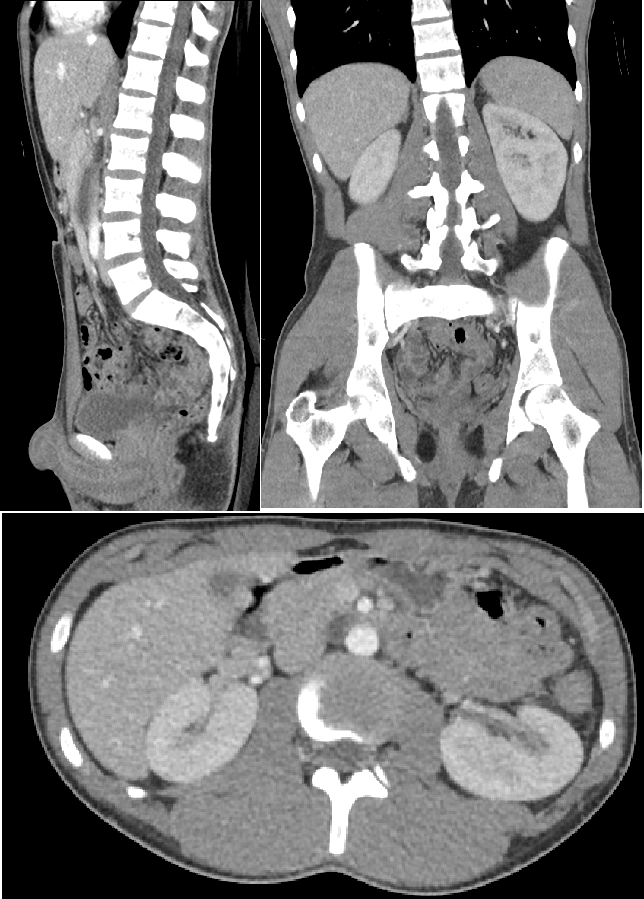
\includegraphics[width=4.5cm]{CT_of_a_normal_abdomen_and_pelvis} % https://upload.wikimedia.org/wikipedia/commons/2/2b/CT_of_a_normal_abdomen_and_pelvis%2C_thumbnail.png
\end{flushright}

\section{History}
\begin{itemize}
\item \popup{Computed Tomography (CT)}{tomografía axial computarizada (TAC)} is a medical imaging modality that became
clinically available in the early 1970s and was the first to be made
possible by computers.
\end{itemize}
\vspace{-3ex}
\begin{figure}[h!]
  \centering
  \begin{tabular}{cc}
    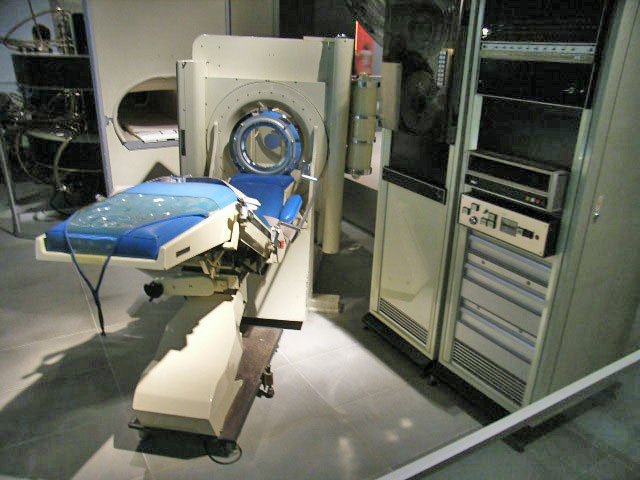
\includegraphics[width=6cm]{Emi1010} &
                                           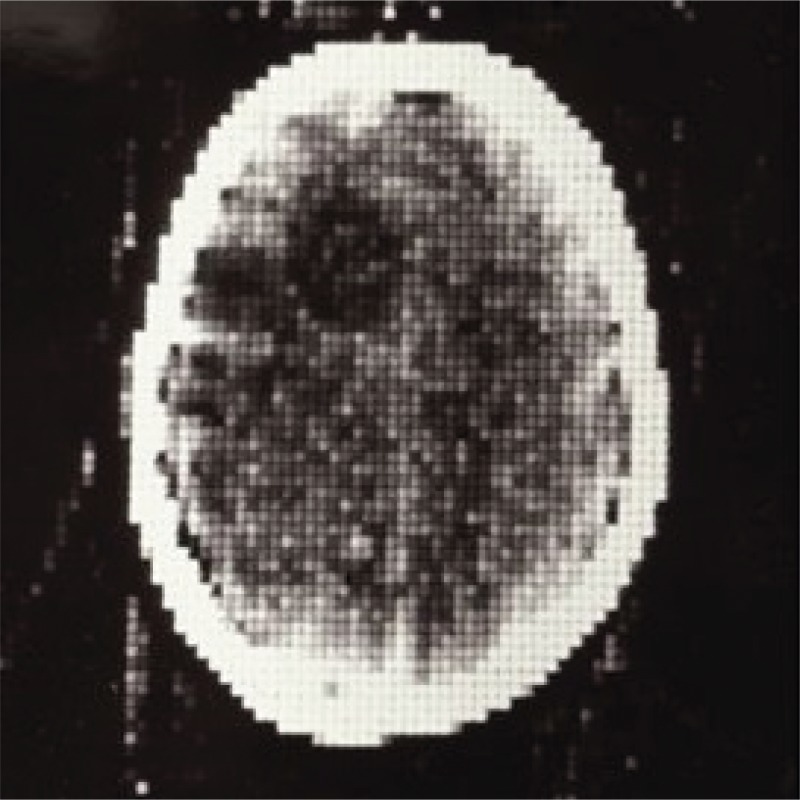
\includegraphics[width=4.5cm]{First_CT_scan_brain}
  \end{tabular}
  \caption{First CT scanner, and an example (80x80 pixels)
    \cite{Wikipedia_CT_history}.\label{fig:first_CT}}
\end{figure}

\section{The CT scanner}
\begin{itemize}
\item The images are obtained by X-ray transmission, moving an X-ray
  tube (the \emph{gantry}, see Fig.~\ref{fig:CT_equipment_machine})
  and detector arrays around the patient.
\end{itemize}
\vspace{-3ex}
\begin{figure}[h!]
  \centering
  \begin{tabular}{cc}
    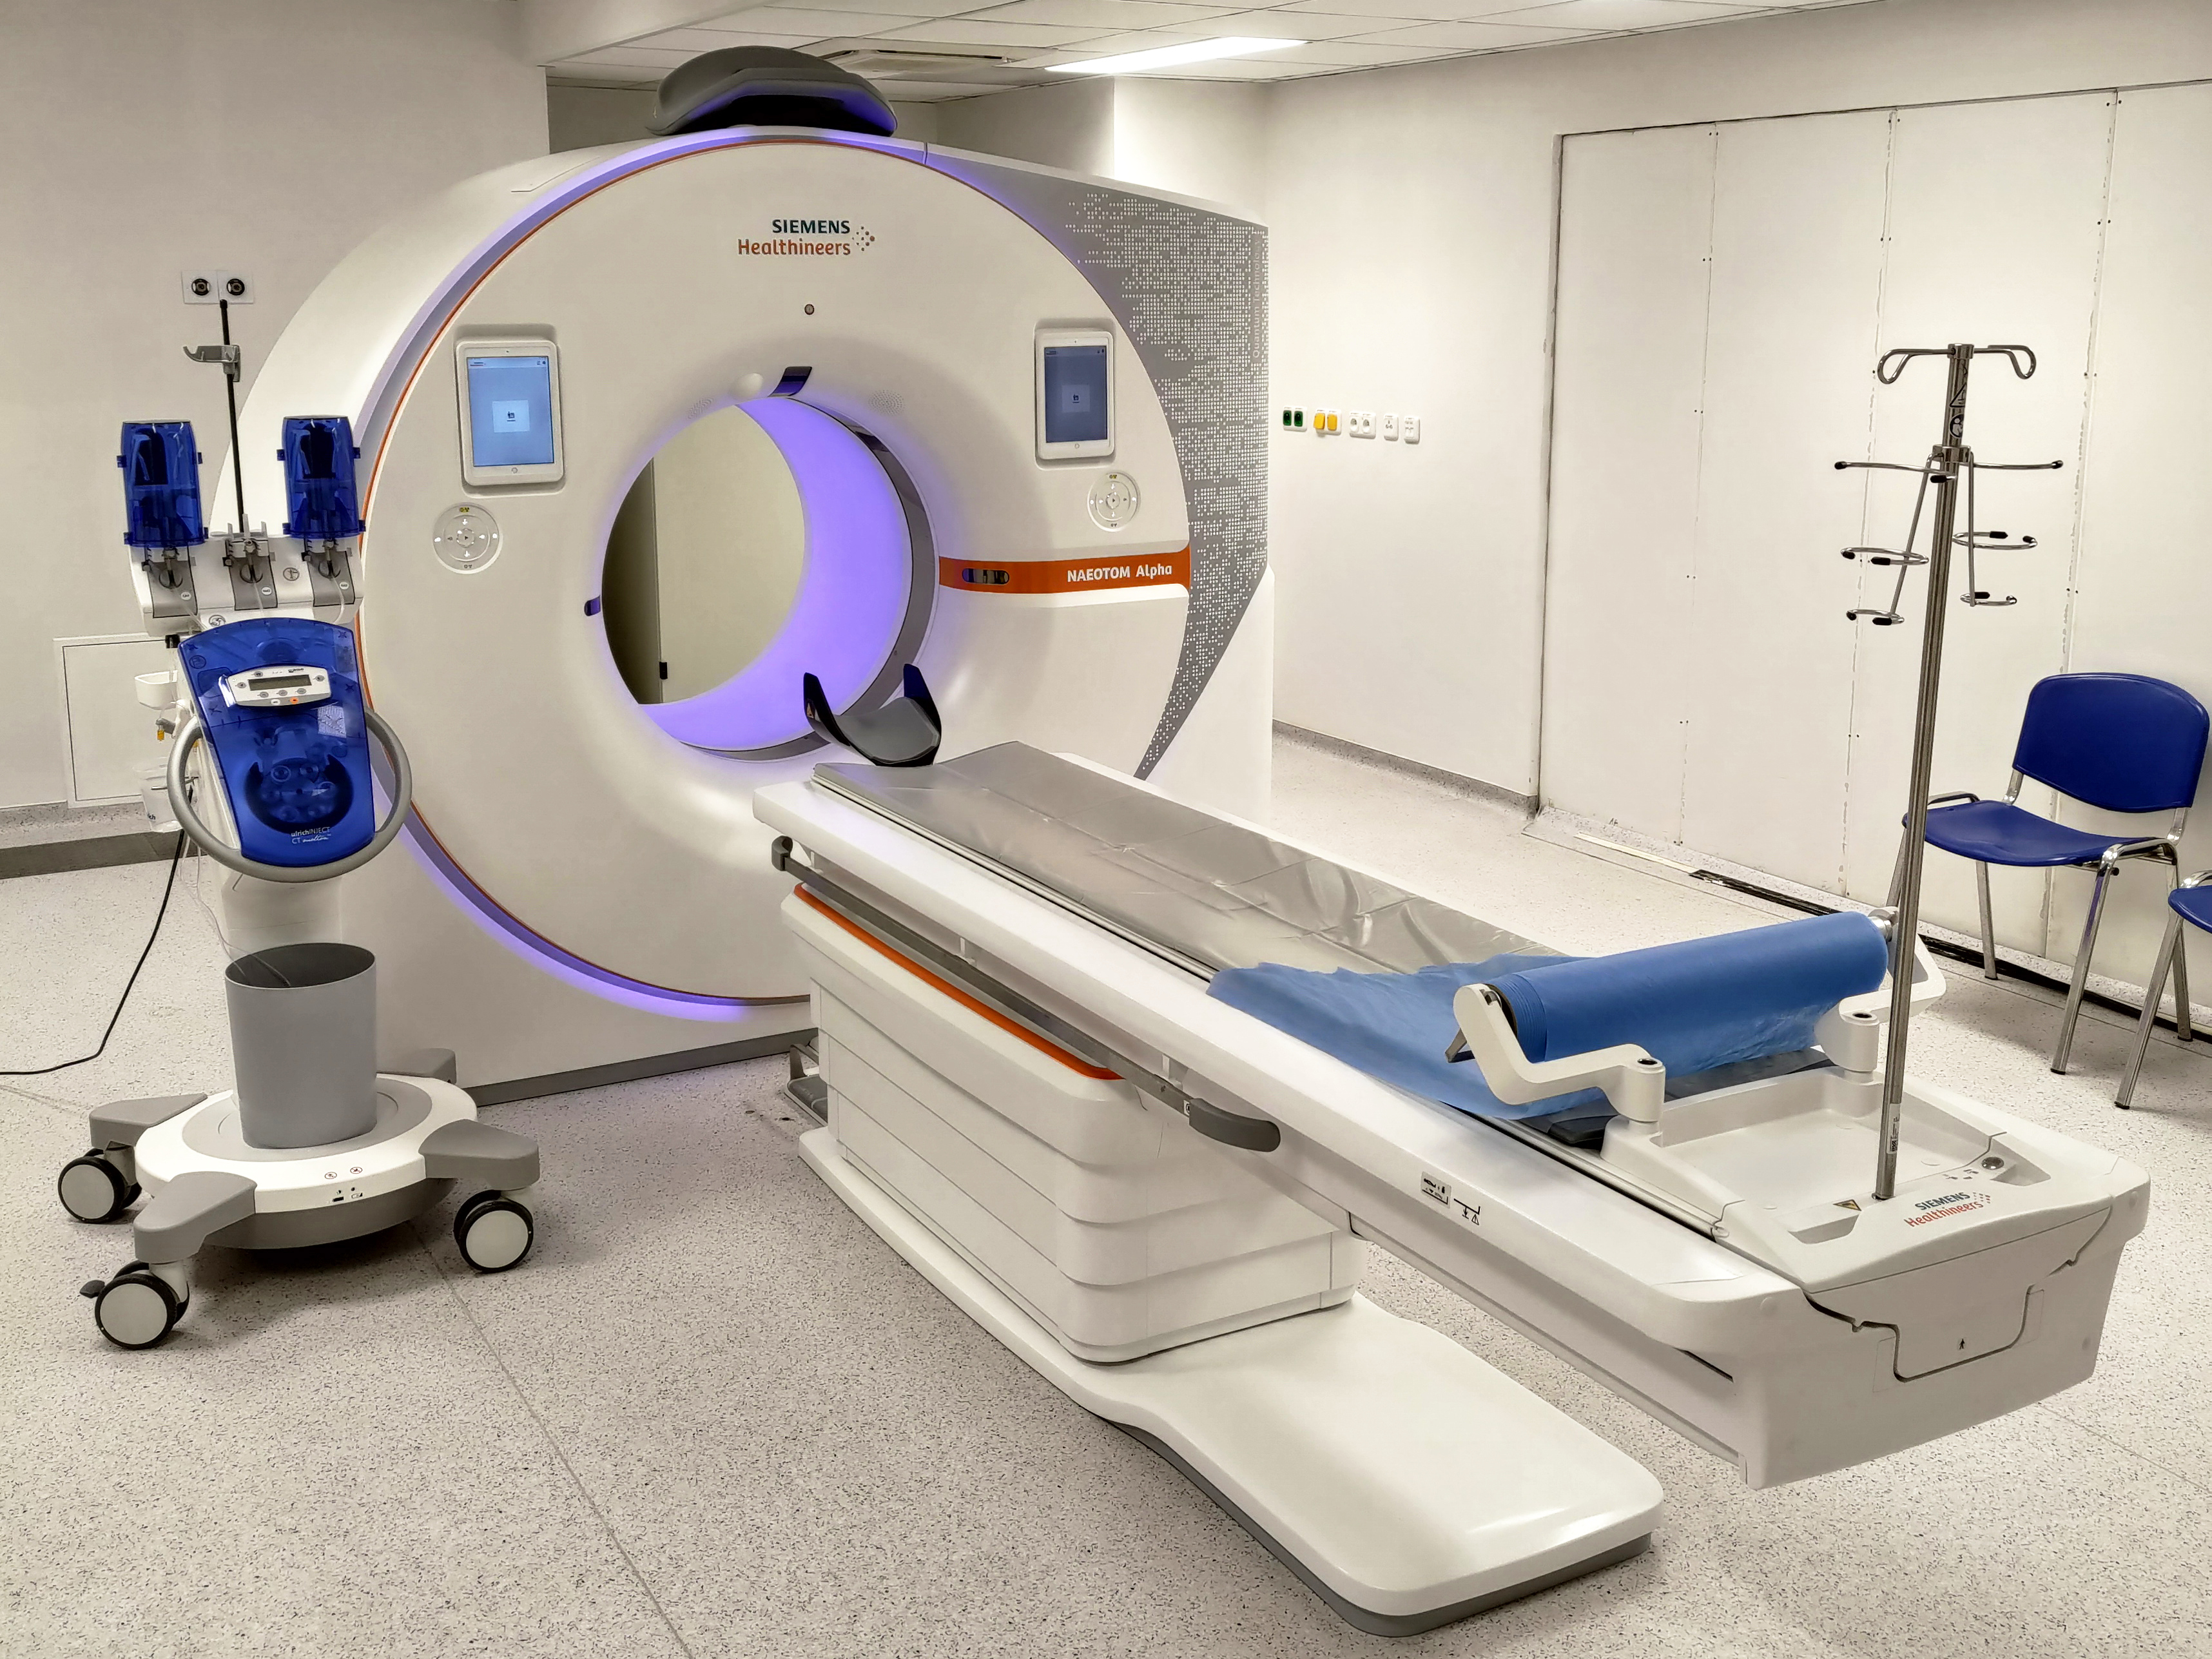
\includegraphics[width=6cm]{CT_Naeotom_Alpha_Pilsen_2022} &
                                                                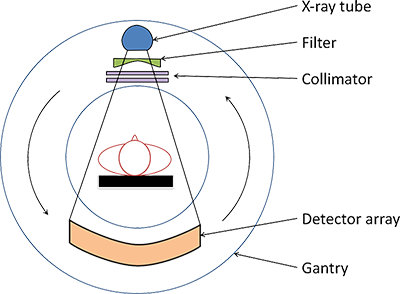
\includegraphics[width=6cm]{CT_equipment_machine}
                                                                \end{tabular}
  \caption{A recent CT scanner and its basic schema \cite{Wikipedia_CT_history}.\label{fig:new_CT}}
\end{figure}

\section{Capabilities}
\begin{itemize}
\item CT can provide \popup{isotropic}{Isotropic spatial resolution is
    a characteristic of images where the resolution is equal in all
    directions. In the case of 3D images, this means that a voxel (a
    3D pixel) is a perfect cube, with equal dimensions on all sides.:
    along the X-axis (left-right), the Y-axis (up-down), and the
    Z-axis (front-back).} 3D images (volumes), including
  \popup{axial}{An axial view divides the body horizontally into a top
    (superior) and bottom (inferior) section.}, \popup{coronal}{A
    coronal view divides the body vertically into a front (anterior)
    and back (posterior) section.}, and \popup{sagittal}{A sagittal
    view divides the body vertically into a right and left section.}
  views (see Fig.~\ref{fig:views_in_CT}).
\item The use of
  iodinated contrast injected intravenously allows the functional
  assessment of various organs as well \cite{bushberg2011essential}.
\end{itemize}
\vspace{-4ex}
\begin{figure}[!b]
  \centering
  \begin{tabular}{cc}
    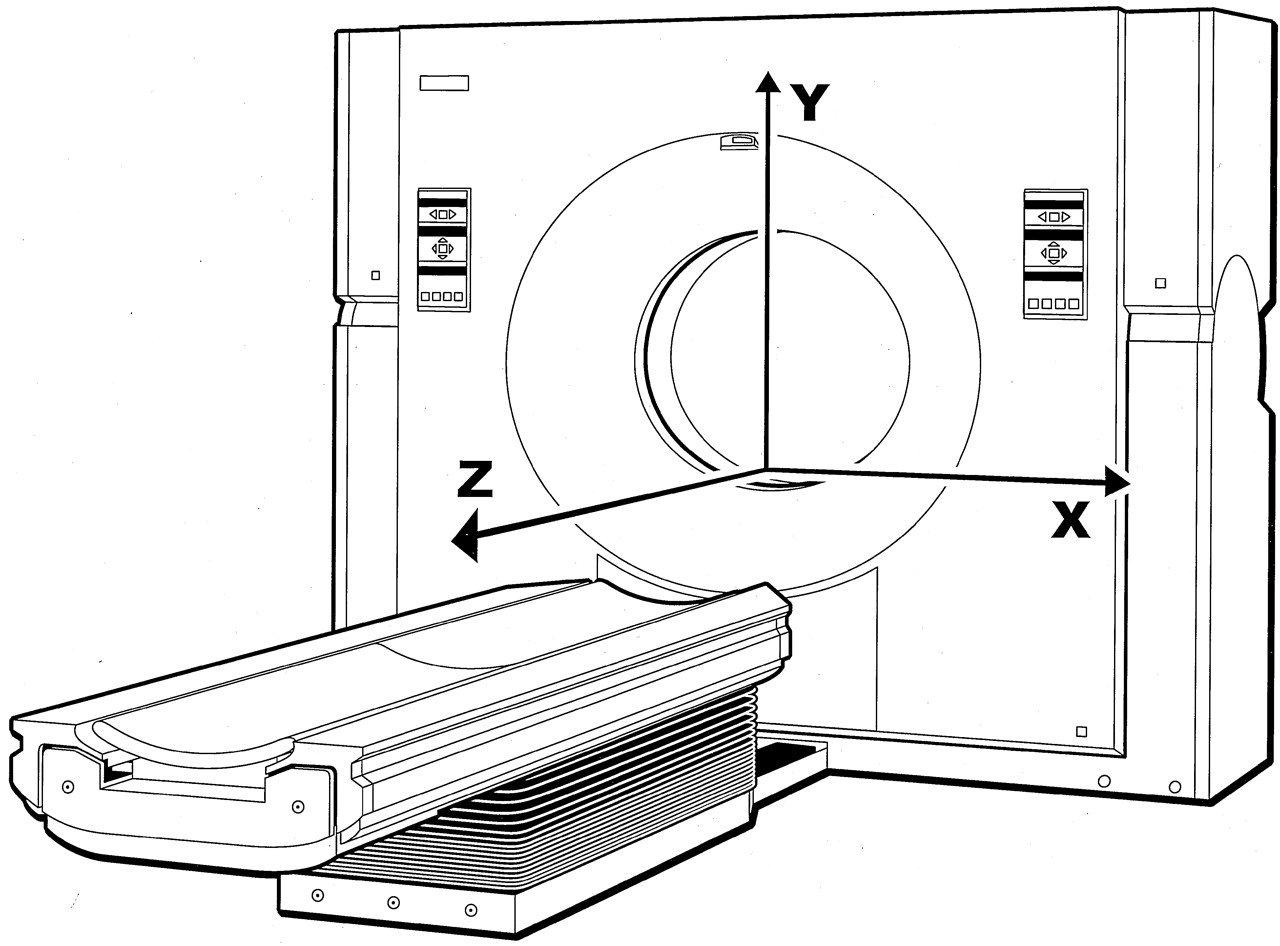
\includegraphics[height=3.5cm]{CT_axis} & 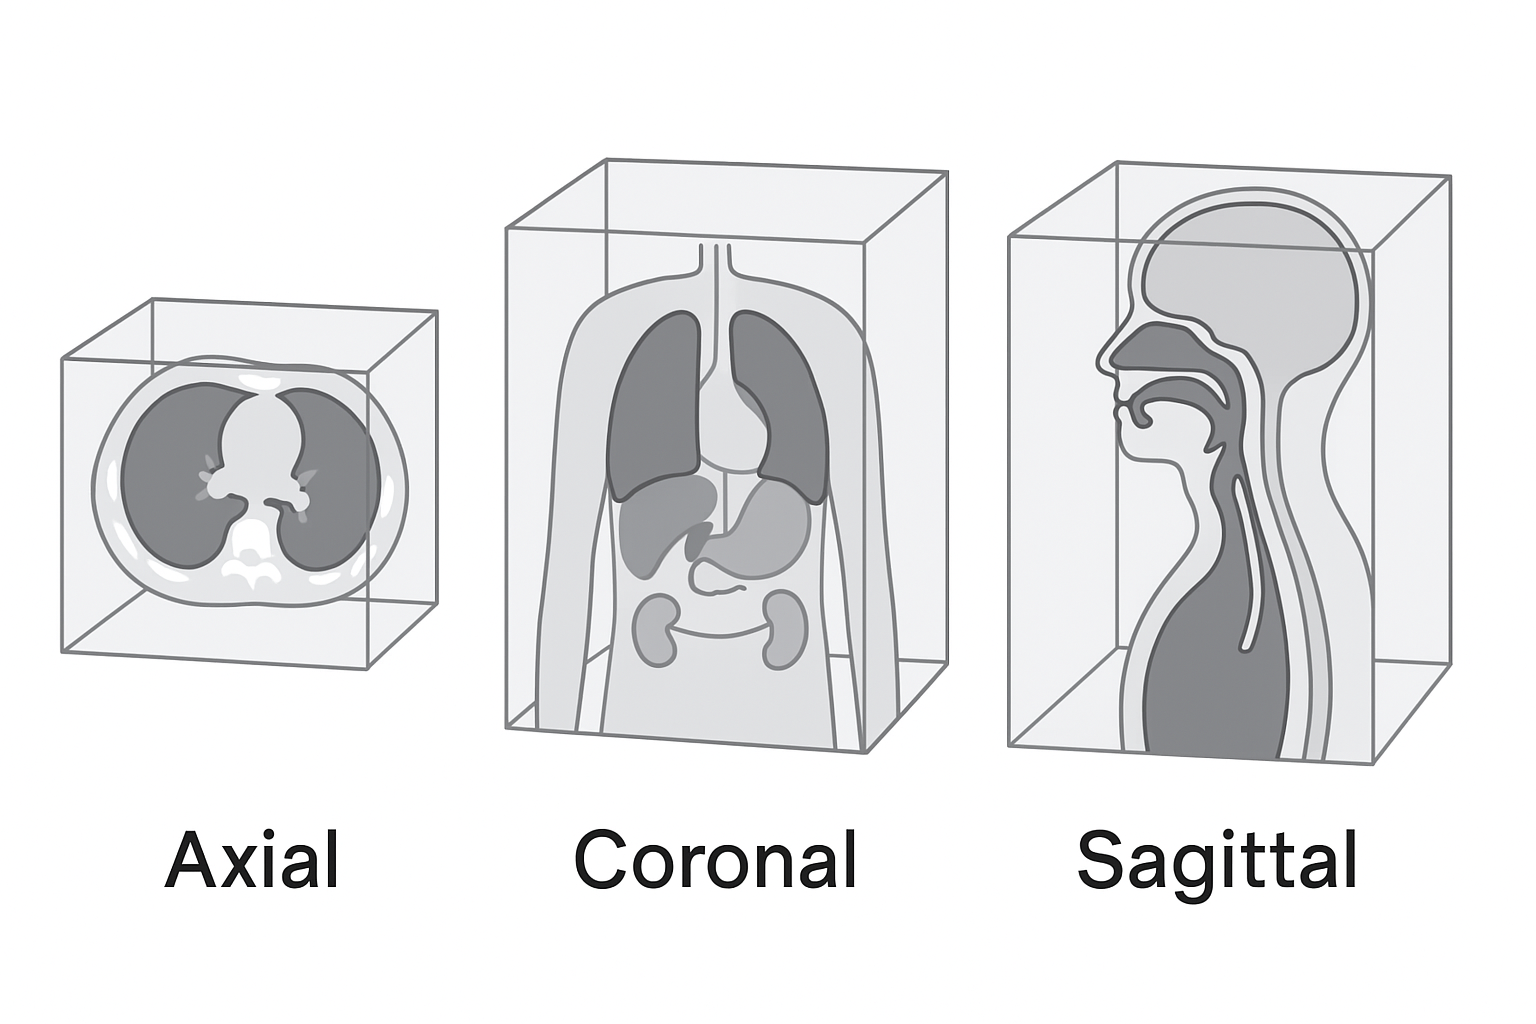
\includegraphics[height=4cm]{axial_coronal_sagittal}
  \end{tabular}
  \caption{Reference axis used in CT and views generated
    \cite{morin2025radiation}.\label{fig:views_in_CT}}
\end{figure}

\section{Acquisition (1/3)}
\begin{itemize}
\item The 2D data collected from each angle is called a \emph{projection}
(see Fig.~\ref{fig:projection}), consisting of multiple individual
attenuation measurements.
\end{itemize}
\vspace{-5ex}
\begin{figure}[!b]
  \centering
  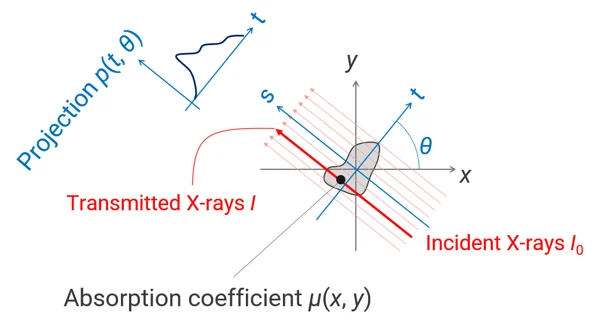
\includegraphics[height=4.5cm]{projection}
  \caption{A projection example \cite{takase2025CT}. $\theta$ is the
    angle used for taking the projection and $t$ the location in
    the detector.\label{fig:projection}}
\end{figure}

\section{Acquisition (2/3)}
\begin{itemize}
\item The acquisition process can be classified as
(see Fig.~\ref{fig:CT_geometries}):
\begin{enumerate}
\item \textbf{Parallel-beam}: The X-rays are parallel and the detector
  is organized as a 1D array.
\item \textbf{Fan-beam}: The X-rays form a fan with the vertice in the
  emitter in a line and the detector is organized as a 1D array.
\item \textbf{Cone-beam}: The X-rays form a cone with the
  vertice in the emitter, and the detector is a 2D array.
\end{enumerate}
\end{itemize}
\vspace{-5ex}
\begin{figure}[!b]
  \centering
  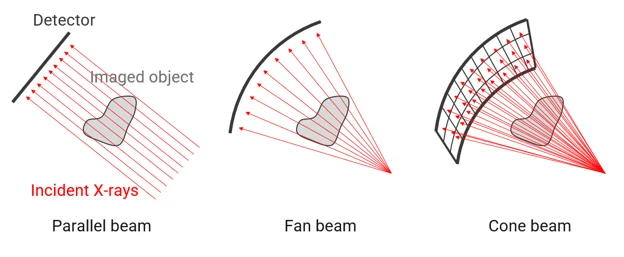
\includegraphics[height=3.2cm]{CT_geometries}
  \caption{Acquisition geometries used in CT \cite{takase2025CT}.\label{fig:CT_geometries}}
\end{figure}

\section{Acquisition (3/3)}
\begin{itemize}
\item Depending on how the scanning is performed, we can distinguish between
(see Fig.~\ref{fig:scannings}):
\begin{enumerate}
\item \textbf{Axial (sequential) scanning}:
  The gantry completes a 360-degree rotation to acquire projection
  data while the patient table is stationary. 
\item \textbf{Helical (spiral) scanning}: The patient table moves
  at a constant speed while the gantry rotates, causing the X-rays
  source to form a helix around the patient.
\end{enumerate}
\end{itemize}
\begin{figure}[!b]
  \centering
  \begin{tabular}{cc}
    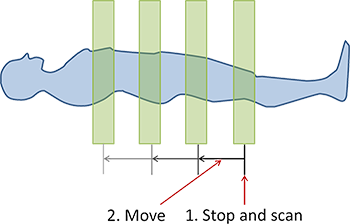
\includegraphics[height=3cm]{axial_scanning} & 
\includegraphics[height=3cm]{helical_scanning}
  \end{tabular}
  \caption{Types of scanning used in CT \cite{abdulla2025acquiring1}.\label{fig:scannings}}
\end{figure}

\section{Sinogram (1/2)}
\begin{itemize}
\item In parallel- and fan-beam scaners, the projections
  are (1D) lines and the set of all projections for the same Z-plane
  form a 2D image called \popup{\emph{sinogram}}{The Radon transform
    describes how CT projections are mathematically related to the
    scanned object. Back-projection is the reconstruction method that
    (with filtering) approximates the inverse Radon transform to
    recover the object from its projections.}. In cone-beam scaners,
  the sinogram is a 3D cube \cite{wikipedia2025radom_transform}.
\end{itemize}
\vspace{-3ex}
\begin{figure}[!b]
  \centering
  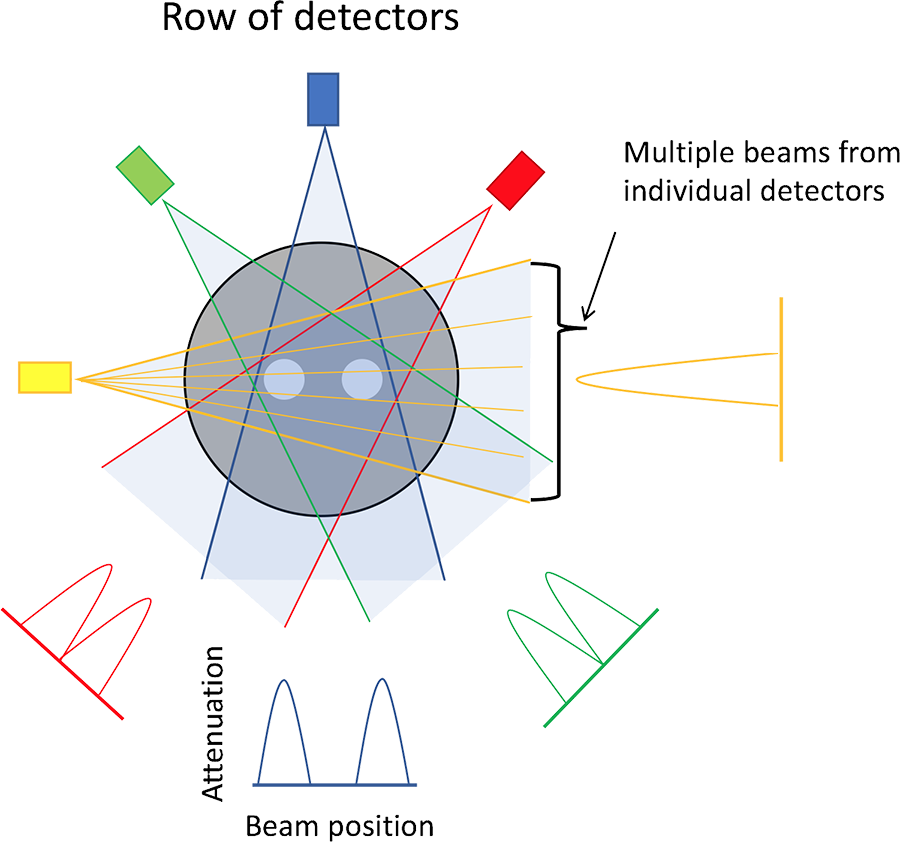
\includegraphics[height=4.5cm]{sinogram_generation}
  \caption{Sinogram generation example
    \cite{abdulla2025acquiring2}.\label{fig:sinogram_generation}}
\end{figure}

\section{Sinogram (2/2)}
\begin{itemize}
\item The CT scaner generates a \popup{collection}{usually thousands}
  of projections that need to be processed to obtain the 3D
  reconstruction. See this
  \href{https://en.wikipedia.org/wiki/Radon_transform#/media/File:Radon_transform_sinogram.gif}{GIF
    sinogram example}.
\end{itemize}
\vspace{-3ex}
\begin{figure}[!b]
  \centering
  \begin{tabular}{cc}
    
\includegraphics[height=4cm]{Two_Squares_Phantom} & 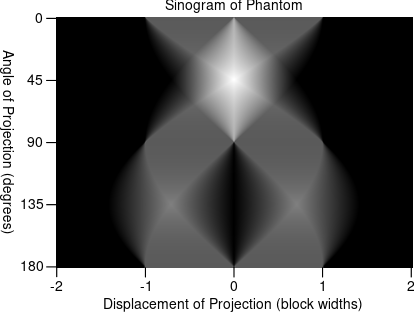
\includegraphics[height=4cm]{Sinogram_-_Two_Square_Indicator_Phantom}
  \end{tabular}
  \caption{a 2D phatom (left) and its sinogram (right)
    \cite{wikipedia2025radom_transform}.\label{fig:sinogram_phantom}}
\end{figure}

\section{Tomogram reconstruction}
\begin{itemize}
\item A \popup{tomogram}{A 2D structure.} is the resulting 2D
  reconstruction of an \popup{slice}{A 2D structure.} scanned
  object by means of its \popup{sinogram}{A 2D structure}.
\item Tomograms can be reconstructed in the spatial domain (using the
  Filtered Back-Projection algorithm or iterative algorithms) and in
  the frequency domain (using the Radon transform).
\end{itemize}

\section{Filtered Back-Projection (FBP) (1/2)}
\begin{itemize}
\item The tomogram structure accumulates in each voxel the
  constribution of each projection \cite{abdulla2025acquiring2} (see
  Figure~\ref{fig:CT_reconstruction})), that previously has been
  \popup{filtered}{The filtering is usually performed in the Fourier
    domain, where the convolution is a linear-time operation. The FFT
    (Fast Fourier Transform, both forward and inverse) requires
    n log2(n)) operations and the multiplication requires
    n operations, where n is the number of elements to
    convolve. Convolution in the signal domain requires
    n^2. Therefore, the projections must be FFT-transformed
    (n log2(n)), perform the point-wise multiplication
    (n), and inverse FFT-transformed
    (n log2(n)). Therefore, for large enough $n$,
    convolution in the Fourier domain is faster.} using a high-pass
  filter to sharpen the textures of the reconstruction.
\end{itemize}

\section*{Filtered Back-Projection (FBP) (2/2)}
\vspace{-2ex}
\begin{figure}[!b]
  \centering
  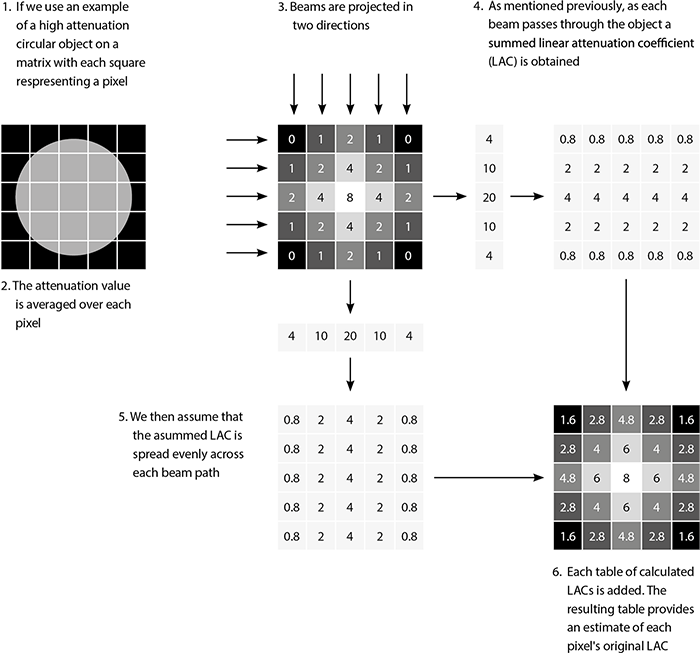
\includegraphics[height=6cm]{CT_backprojection}
  \caption{An example of reconstruction with FBP using only 2
    projections
    \cite{abdulla2025acquiring2}.\label{fig:CT_reconstruction}}
\end{figure}

\section{Iterative algorithms}
\begin{itemize}
\item Handle noise and incomplete data better but require more computation.
\item Basic algorithm:
  \begin{enumerate}
  \item Start with an initial guess of the image (for example obtained with FBP).
  \item Simulate what projections this guess would produce.
  \item Compare with the measured projections.
  \item Update the guess to reduce the error.
  \item Repeat until convergence.
  \end{enumerate}
\item Examples: ART (Algebraic Reconstruction Technique), SIRT
  (Simultaneous Iterative Reconstruction Technique), and modern
  statistical or model-based methods.
\end{itemize}

\section{Radon transform}
\begin{itemize}
\item The Radon transform models how a sinogram is generated. In other
  words, the Radon transform of an \popup{image}{In the context of CT,
    the input image is the tomogram that we want to reconstruct.} is
  its sinogram.
\item The inverse Radon transform, by definition, inputs a sinogram
  and outpus the original image.
\end{itemize}

\section{FFT-based inverse Radon transform (1/2)}
\begin{itemize}
\item The reconstruction of a tomogram using the Radon transform can
  run faster (using the \popup{FFT}{The FFT (Fast Fourier Transform)
    is a fast algorith to ``travel'' between the signal domain and the
    frequency domain.}) with the following algorithm:
  \begin{enumerate}
  \item Compute the FFT of each projection, resulting a new sinogram
    where each row is in the frequency domain.
  \item Distribute each row in a circle (a image), depending on the
    angle at which each projection was taken.
  \item Compute the inverse 2D-FFT of the circle.
  \end{enumerate}
\end{itemize}
\vspace{-4ex}
\begin{figure}[!b]
  \centering
  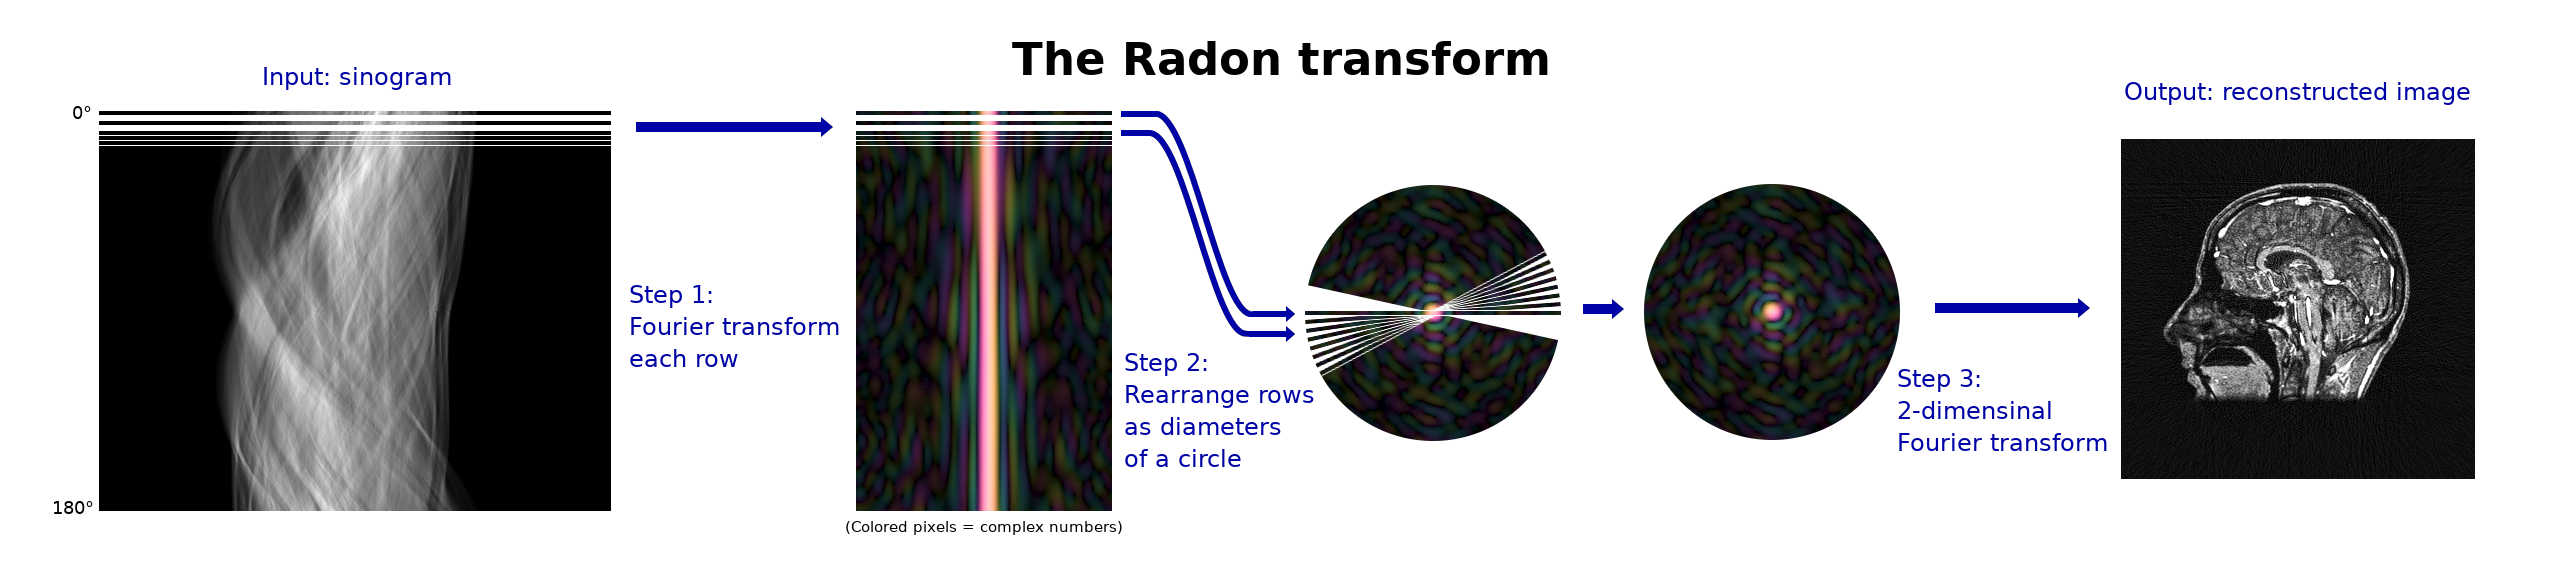
\includegraphics[width=0.8\textwidth]{Radon_transform_via_Fourier_transform}
  \caption{The inverse Radon transform using the frequency domain
    \cite{wikipedia2025radom_transform}.\label{fig:inverse_Radon}}
\end{figure}

\section{Volume reconstruction}
\begin{itemize}
\item The 3D volume is form by the stacking of all 2D tomograms.
\end{itemize}

\section{Radon transform and Fourier transform}



To generate the 3D reconstruction, the following tasks are usually done:


\begin{enumerate}
\item \textbf{Calibration}: A phantom patient (that we know exactly
  its morphology) is used to test if the reconstructions have some
  problem, such as for example, the detector sensitivity (affects to
  the contrast), ``dead-pixels'' in the detector (that should be
  interpolated), etc. This task should bezz performed periodically.
\item \textbf{Denoising}: The sinograms used to be quite
  smooth. Therefore, some technique for removing noise can be
  useful. This task is performed in every scan.
\item \textbf{Logarithmic transformation}: The X-rays are
  exponentially attenuated when they travel across the tissues. This
  step generates LACs (Linear Attenuation Coefficient), and allows to
  suppose that the rest of tasks are using linear data.
\item \textbf{Filtered BackProjection (FBP)}: 

  Alternatively, instead of FBP an (usually ``heavier'') iterative
  reconstruction algorithm can be used.\footnote{These algorithms
    start with an initial guess of the image, calculate forward
    projections, compare them to the actual measured projection data
    to generate an "error matrix," and then use this error to update
    the image in successive iterations until an accurate depiction of
    the scanned object is achieved.}

\end{enumerate}

\section{Quantum noise}

The processes by which radiation is emitted and interacts with matter
are inherently random, making all radiation measurements, including
medical imaging, subject to random error. The Poisson distribution is
particularly relevant to quantum noise in radiological imaging. The
noise per pixel ($\sigma$) is approximated by the square root of the
mean number of photons ($N$) recorded in each detector element, i.e.,
$\sigma = \sqrt{N}$ \cite{bushberg2011essential}.

In CT, quantum noise tends to dominate at high spatial frequencies in
the projection data, which can lead to unacceptably noisy
reconstructed images if appropriate filtering is not applied
\cite{bushberg2011essential}.

